\Problem{Springloaded Sled}{\SpringSled}{
You are designing a sled with a compressed spring inside, which can be released to separate the sled into two pieces of equal mass ($m/2$). You are racing the sled across level snow at speed $v$ when you trigger the separation.
%A firework is moving to the right with speed v when it explodes into two pieces with equal mass (m/2).
}
\ProblemSub{\SpringSledMomEn}{
Right after the two halves push apart, the back end of the sled is moving backward with speed $v$. What is the velocity of the other piece? How much kinetic energy did the system gain?
%Right after the explosion, the first piece is moving backward with speed v.
%What is the velocity of the other piece?
%How much kinetic energy did the system gain?
}
\ProblemFig{\SpringSledFig}{
\centering
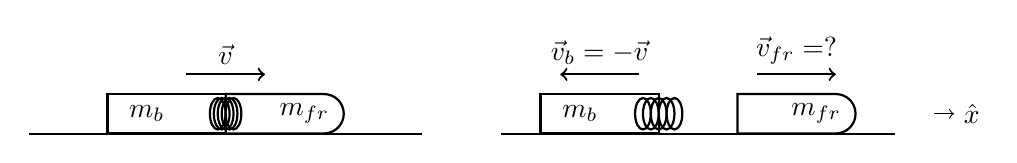
\begin{tikzpicture}
	\begin{scope}[rotate=0,shift={(-3,0)}]
		\draw[thick,->] (-0.5,0.5) -- (0.5,0.5);
		\node[anchor=south] at (0,0.5) {$\vec{v}$};
		\begin{scope}
			\draw[thick] (-1.5,0.25) rectangle (0,-0.25);
			\node at (-1,0) {$m_{b}$};
		\end{scope}
		\begin{scope}
			\draw[thick] (0,0.25) -- (1.25,0.25) arc (90:-90:0.25) -- (0,-0.25) -- cycle;
			\node at (1,0) {$m_{fr}$};
		\end{scope}
		\begin{scope}[yscale=2]
			\newcommand{\Comp}{0.05}
			\draw[thick] ({-\Comp*2},0) circle (0.1);
			\draw[thick] (-\Comp,0) circle (0.1);
			\draw[thick] (0,0) circle (0.1);
			\draw[thick] (\Comp,0) circle (0.1);
			\draw[thick] ({\Comp*2},0) circle (0.1);
		\end{scope}
		\draw[thick] (-2.5,-0.26) -- (2.5,-0.26);
	\end{scope}
	\begin{scope}[rotate=0,shift={(3,0)}]
		\begin{scope}[shift={(-0.5,0)}]
			\draw[thick,->] (-0.25,0.5) -- (-1.25,0.5);
			\node[anchor=south] at (-0.75,0.5) {$\vec{v}_{b}=-\vec{v}$};
			\draw[thick] (-1.5,0.25) rectangle (0,-0.25);
			\node at (-1,0) {$m_{b}$};
		\end{scope}
		\begin{scope}[shift={(0.5,0)}]
			\draw[thick,->] (0.25,0.5) -- (1.25,0.5);
			\node[anchor=south] at (0.75,0.5) {$\vec{v}_{fr}=$?};
			\draw[thick] (0,0.25) -- (1.25,0.25) arc (90:-90:0.25) -- (0,-0.25) -- cycle;
			\node at (1,0) {$m_{fr}$};
		\end{scope}
		\begin{scope}[yscale=2,shift={(-0.5,0)}]
			\newcommand{\Comp}{0.1}
			\draw[thick] ({-\Comp*2},0) circle (0.1);
			\draw[thick] (-\Comp,0) circle (0.1);
			\draw[thick] (0,0) circle (0.1);
			\draw[thick] (\Comp,0) circle (0.1);
			\draw[thick] ({\Comp*2},0) circle (0.1);
		\end{scope}
		\draw[thick] (-2.5,-0.26) -- (2.5,-0.26);
	\end{scope}
	\begin{scope}[shift={(6,0)}]
		\draw[->] (0,0) -- (0.25,0);
		\node[anchor=west] at (0.25,0) {$\hat{x}$};
	\end{scope}
\end{tikzpicture}
}
\Solution{\SpringSledSol}{
	
When setting up a motion vector diagram for this problem, I know the initial momentum of the combined sled system, and I know both parts of the sled have half of this momentum. I also know that the final momentum of the back half is reversed, and the total momentum of the system is unchanged, so I can infer the rest of the table from there.
\begin{figure}[h]
	\centering
	\begin{tikzpicture}
		\MVDRows{MVD}
		\MVDCol{mass}{Back}{MVD}{0.75}
		\MVec{massinit}{0.3}
		\MVec[180]{massdelt}{0.6}
		\MVec[180]{massfin}{0.3}
		\MVDCol{Mass}{Front}{mass}{0.75}
		\MVec{Massinit}{0.3}
		\MVec{Massdelt}{0.6}
		\MVec{Massfin}{0.9}
		\MVDCol{sys}{Both}{Mass}{0.75}
		\MVec{sysinit}{0.6}
		\MDot{sysdelt}
		\MVec{sysfin}{0.6}
	\end{tikzpicture}
\end{figure}

The initial momentum of the system is $mv\hat{x}$, and the final momentum is $(\frac{m}{2}v_{fr}-\frac{m}{2}v)\hat{x}$. Since the momentum is conserved (no friction, and the normal force and gravitational force are in balance, so no other net impulse), we know that
\begin{align*}
	mv\hat{x} & = \left(\frac{m}{2}v_{fr}-\frac{m}{2}v\right)\hat{x} \\
	mv & = \frac{m}{2}v_{fr}-\frac{m}{2}v \\
	2v & = v_{fr} - v \\
	v_{fr} & = 3v.
\end{align*}
The front half of the sled gets launched forward at triple its original speed!

As for kinetic energy, the system started with $K_{i} = \frac{1}{2}mv^{2}$, and now it has
\[
K_{f} = \frac{1}{2}\frac{m}{2}v^{2} + \frac{1}{2}\frac{m}{2}(3v)^{2} = \frac{5}{2}mv^{2},
\]
therefore the change in kinetic energy is
\[
\Delta K = K_{f}-K_{i} = 2mv^{2}.
\]

This came from the spring. If the spring constant is $k$ and the spring was compressed by a length $\Delta x$, then we have
\begin{align*}
\frac{1}{2}k\Delta x^{2} & = 2mv^{2} \\
k\Delta x^{2} & = 4mv^{2}.
\end{align*}
This has some interesting design implications. For example, say each half of our sled is 100 kg (say that accounts for the machinery and the load of a single passenger on each half) and its initial speed was a lazy 1 m/s. That would mean the spring has to store 400 J of energy. If $\Delta x = 0.5$ m (which may be too much of a compression for a reasonable use of Hooke's law), then $k=3200$ N/m (or 32 N/cm), which is a pretty stiff spring. If we cannot get a spring this stiff, then we need more compression, but if we cannot obtain a spring that compresses far enough without permanently deforming, then we need it stiffer. The key will be finding the perfect middle ground. It is also worth considering whether having only a single spring is the best option.
}